\documentclass[12pt,a4paper,danish,oneside]{book}
\setlength{\headheight}{15pt}
\usepackage{amsmath, amsthm, amssymb}
\usepackage[framemethod=default]{mdframed}
\usepackage{showexpl}
\usepackage{gensymb}

\mdfdefinestyle{exampledefault}{%
	rightline=true,innerleftmargin=10,innerrightmargin=10,
	frametitlerule=true,frametitlerulecolor=green,
	frametitlebackgroundcolor=yellow,
	frametitlerulewidth=2pt}

\usepackage{lipsum}
\usepackage[framed,numbered,autolinebreaks,useliterate]{mcode}
\usepackage{url,textcomp}
\usepackage{graphicx}
\usepackage[danish]{babel}
\usepackage[utf8]{inputenc}
\usepackage{siunitx}
\usepackage{caption}
\usepackage{float}
\usepackage{pdfpages}
\usepackage[footnote,draft,danish,silent,nomargin]{fixme}

\newmdtheoremenv{exmp}{Example}[section]
\newtheorem{prob}{Problem}[section]
\setcounter{section}{1}


\usepackage{titlesec}
\titleformat{\chapter}[display]
{\normalfont\bfseries\filcenter}
{}
{1ex}
{\titlerule[2pt]
\vspace{2ex}%
\LARGE}
[\vspace{1ex}%
{\titlerule[2pt]}]


\usepackage{cancel}
\usepackage[margin=4cm]{geometry}
\usepackage[hidelinks]{hyperref}
\usepackage{fancyhdr}
\pagestyle{fancy}
\fancyhead{}
\fancyfoot{}
\lhead{ETHFE}
\rhead{\textsc{Jonas Lind}}
\cfoot{\thepage}
    
\newcommand{\HRule}{\rule{\linewidth}{0.5mm}}



\title{ETHFE - High Frequency Electronics}
\begin{document}
\begin{titlepage}
	\clearpage\thispagestyle{empty}

	\begin{center}
		\HRule \\[0.4cm]
		{\huge \bfseries ETHFE} \\[.3cm] {\huge High Frequency Electronics}\\[0cm]
		\HRule \\[3.4cm]
		
\includegraphics[width=0.5\linewidth]{graphics/au}
	\end{center}
	\renewcommand{\contentsname}{Indholdsfortegnelse}
	\tableofcontents

\end{titlepage}

 
%-----------------------------------------------------------------
%   TITLE SECTION
%-----------------------------------------------------------------

\chapter{Amplitude modulation}
\section{Lektion 15-02-2018}
\subsection{GraphicTFT display driver}

Driver for "ITDB02 320 x 240 TFT display module, Version 2" mounted at "ITDB02 Arduino Mega2560 Shield".\\

\noindent Display controller = ILI 9341.\\

\begin{tabular}{ll}
	\textbf{Connections}\\
	\hline
	\rule{0pt}{5mm}  
	DB15-DB8:   & PORT A\\ 
	\rule{0pt}{5mm}
	DB7-DB0:    & PORT C\\ 
	\rule{0pt}{5mm}
	RESETx:     & PORT G, bit 0\\ 
	\rule{0pt}{5mm}
	CSx:        & PORT G, bit 1\\ 
	\rule{0pt}{5mm}
	WRx:        & PORT G, bit 2\\ 
	\rule{0pt}{5mm}
	RS (=D/Cx): & PORT D, bit 7\\ 
\end{tabular} 

\begin{minted}{c}
// Data port definitions:
#define DATA_PORT_HIGH PORTA
#define DATA_PORT_LOW  PORTC

// Control port definitions:
#define WR_PORT PORTG
#define WR_BIT 2
#define DC_PORT PORTD
#define DC_BIT  7  // SHIELD RS
#define CS_PORT PORTG
#define CS_BIT  1
#define RST_PORT PORTG
#define RST_BIT 0
\end{minted}
Start by implementing the basic, time-critical functions.

\begin{figure} [H]
	\centering
	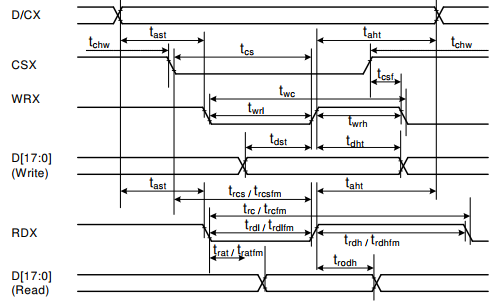
\includegraphics[width=0.8\linewidth]{graphics/LAB3a.png}
	\caption{Timing Characteristics (8080-Ⅰ system).}
	\label{fig:11}
\end{figure}

\noindent\mintinline{c}{PORTD &= ~(1 << n);} will set PIN n low.\\

\noindent\mintinline{c}{PORTD |= (1 << n);} will set PIN n high.

\begin{minted}{c}
void WriteCommand(unsigned int command)
{
DATA_PORT_LOW = command;
DC_PORT &= ~(1<<DC_BIT);       // DCX LOW = COMMAND MODE
CS_PORT &= ~(1<<CS_BIT);       // CSX LOW
WR_PORT &= ~(1<<WR_BIT);       // WRX LOW
_NOP();			// DELAY = twrl 15ns
WR_PORT |= (1<<WR_BIT);	// WRX HIGH
_NOP();			// DELAY = tcf 10ns
}
\end{minted}

\begin{minted}{c}
void WriteData(unsigned int data)
{
DATA_PORT_HIGH = (data >> 8);	// MSB
DATA_PORT_LOW  = data;	       // LSB
DC_PORT |= (1<<DC_BIT);	      // DCX HIGH = DATA MODE
CS_PORT &= ~(1<<CS_BIT);	     // CSX LOW
WR_PORT &= ~(1<<WR_BIT);	     // WRX LOW
_NOP();			      // DELAY = twrl 15ns
WR_PORT |= (1<<WR_PORT);	     // WRX HIGH
_NOP();			      // DELAY = twcf 10ns
}
\end{minted}

\chapter{Vinkel modulation}
\section{Lektion 08-02-2018}

\begin{enumerate}
	\item Mikrofon
	\item Højtaler (afstandsregel)
	\item Måling af lydtryk
\end{enumerate}

\begin{mdframed}[style=exampledefault]
	\begin{itemize}
		\item \textbf{Pensum:} 
		\begin{enumerate}
			\item Audio Meetering, sec. 8-9, 26-29
			\item Elektroakustik, TAS,  p. 12-14
		\end{enumerate}
		\item \textbf{Opgaver:} 
		\begin{enumerate}
			\item Lyd og Akustik - Lektion 2 - opgaver og øvelser
		\end{enumerate}
	\end{itemize}
\end{mdframed}

\subsection{Mikrofon}
\begin{itemize}
	\item En transducer der omsætter et oscillerende lydtryk til et analogt elektrisk signal.
	\begin{itemize}
		\item Kaldes også for en tryktransducer.
		\item Måler lydtrykkets variation i et punkt uden reference til den retning lyden udbredes i.
		\item Flere mikrofontyper er retningsbestemte på grund af deres opbygning.
	\end{itemize}
\end{itemize}

\subsubsection{Kondensator mikrofon}
\begin{itemize}
	\item En tynd membran af udspændt metalfolie er anbragt tæt på
	en fastsiddende elektrode.
	\item Kondensatoren mellem membran og elektrode oplades gennem $R_p$. 
	\item Spændingen mellem membran og elektrode vil variere efter definitionsligningen $Q = C\cdot U$.
	\begin{itemize}
		\item $Q$ er den konstante ladning givet af polarisationsspændingen $U_P$ der ved målemikrofoner typisk er \SI{200}{\volt}.
	\end{itemize}
	\item Den lave grænsefrekvens sættes af $R_p$ og mikrofonens kapacitet $C$.
	\begin{itemize}
		\item $C \approx \SI{5}{\pico\farad}-\SI{20}{\pico\farad}$ gør at  $R_p$ skal være mindst \SI{1}{\giga\ohm} for måling af hørbar lyd.
	\end{itemize}
	\item Den høje grænsefrekvens sættes af membranens masse. 
\end{itemize}

\begin{figure} [H]
	\centering
	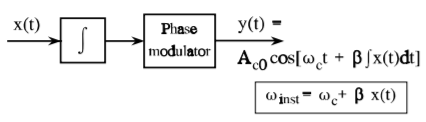
\includegraphics[width=\linewidth]{graphics/11.png}
	\caption{Kondensatormikrofons opbygning.}
	\label{fig:11}
\end{figure}

\begin{itemize}
	\item Alternativt indbygges en plastskive mellem membran og elektrode hvor en såkaldt "fastfrosset ladning" fungerer som $Q$.
	\item Den høje udgangsimpedans sænkes af en indbygget JFET og det eksterne kredsløb skal nu levere strøm til transistorens drain.
	\item Følsomheden er typisk $\approx 5 \si{\milli\volt}/\si{\pascal}$. 
\end{itemize}

\subsubsection{Dynamisk mikrofon}
\begin{itemize}
	\item \textbf{Klassiske form}: minder om en højttaler (membranen sættes i bevægelse af lydtrykket). Derved bevæges svingspolen i magnetfeltet
	og der induceres en spænding.
	\item \textbf{Båndmikrofonen}: membranen er i et kraftigt magnetfelt. Når lydtrykket får membranen til at svinge induceres der en spænding over de to ender af båndet. Spændingen er normalt så lav at der skal benyttes en transformator for at løfte det op på et brugbart niveau. 
	\begin{itemize}
		\item Lyden har adgang til begge sider af membranen.
		\begin{itemize}
			\item Mest følsom for lyd på aksen ($0\degree$ og $180\degree$.
			\item Der kan ikke registreres lyd fra siden ($90\degree$).
		\end{itemize}
	\end{itemize} 
\end{itemize}
\begin{figure} [H]
	\centering
	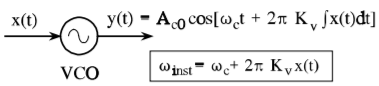
\includegraphics[width=.9\linewidth]{graphics/12.png}
	\caption{(V: svingspolen drives af en membran til at svinge i et magnetfelt.) (H: En tynd metalfolie svinger i et magnetfelt og signalet tages ud ved båndets ender (ud af papiret og ind i papiret)).}
	\label{fig:12}
\end{figure}

\subsection{Højtaler (afstandsregel)}
\fxnote{Mangler højtaler (aftandsregel) noter.}

\subsection{Måling af lydtryk}
\fxnote{Mangler måling af lydtryk noter.}

\subsection{Opgaver}

\begin{enumerate}
	\item Lav et MLS signal med orden 10.
	\item Find impulsresponsen ud fra de sammenhørende exitations- og målesignaler i filen meassigs.mat. Systemet er ”målt” både med MLS og hvid støj.
	\item En 8 ohms højttaler har DC modstand på 6 ohm og virkningsgrad på 1 \%.
	\begin{enumerate}
		\item Bestem den producerede akustiske effekt, når højttaleren tilføres 2,83 volt.
		\item Lyden antages at udbrede sig sfærisk fra højttaleren. Beregn intensiteten og lydtrykniveauet på 2,5 meters afstand.
		\item Lydtrykket måles nu med en mikrofon hvis følsomhed er 5 mV/Pa. Hvilken spænding leverer mikrofonen?
	\end{enumerate}
\end{enumerate}


\begin{lstlisting}
%% LYAK L2 08-02-2018

\end{lstlisting}



\chapter{Parallel og serie resonans kredsløb}
\section{Lektion 15-02-2018}

\begin{enumerate}
	\item Stående bølger
	\item Geometrisk rumakustik
	\item Refleksion
	\item Diffraktion
	\item Statistisk rumakustik
	\item Absorptionskoeffficienter
\end{enumerate}

\noindent\fbox{\parbox{\textwidth}{
	\begin{itemize}
	\item \textbf{Pensum:} 
	\begin{enumerate}
		\item Master Handbook of Acoustics, ch. 6, 7, 11, 13
		\item Elektroakustik, TAS,  p. 89-96
	\end{enumerate}
	\item \textbf{Opgaver:} 
	\begin{enumerate}
		\item Lyd og Akustik - Lektion 4 - opgaver og øvelser
	\end{enumerate}
\end{itemize}
}} \vspace{3mm}

\subsection{Stående bølger}
Et retvinklet rum vil have et system af egenfrekvenser. Her vil plane bølger spejles så de understøtter bestemte frekvenser. Dette sker gennem konstruktiv interferens. \\

\noindent Den laveste frekvens hvor der kan dannes resonans i en akseretning har en bølgelængde på halvdelen af længdedimensionen ($L_x$, $L_y$ og $L_z$). Trykbølgen reflekteres ved væggen og refleksionen kan derfor understøtte den efterfølgende bølgefront.
\begin{itemize}
	\item Ved \SI{5}{\meter} afstand mellem to vægge er den lavest mulige resonans $f_0 = \SI{34}{\hertz}$. Hertil kommer også resonans ved de harmoniske frekvenser på \SI{68}{\hertz}, \SI{102}{\hertz}, ... Tilsvarende gælder for de andre akseretninger.
\end{itemize}
Der er mulighed for stående bølger som involverer fire eller seks vægge.
Dette beskrives ved at to eller tre værdier af index ($n_x$, $n_y$ og $n_z$) er forskellige fra nul. 
De tre indeksværdier kombineres til et enkelt ved at udnytte at N er den højest mulige værdi. Herved kan resonanserne plottes som
funktion af et fælles indeks \textit{n}.\\

\noindent Modellen gælder indtil frekvenser hvor usikkerheden på længderetningen
bliver sammenlignelig med bølgelængden. 
Det kan vises at den øvre grænse er i cirka \SI{550}{\hertz} for
et normalt beboelsesrum hvorved det enkelte indeks er begrænset til området $n = 0$ ... $7$.

\begin{figure} [H]
	\centering
	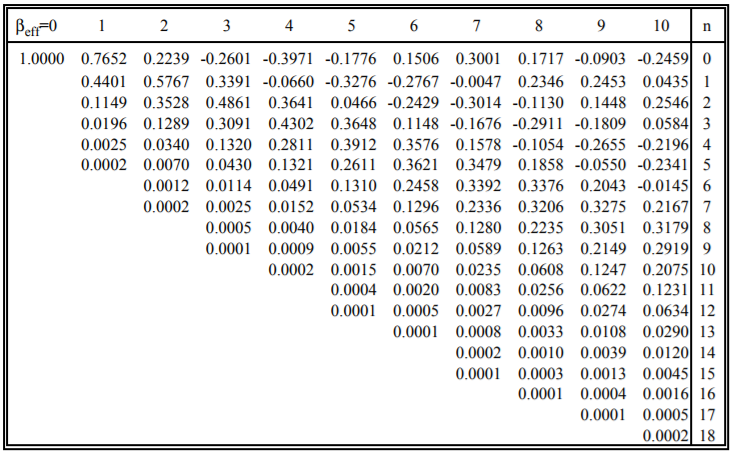
\includegraphics[width=.4\linewidth]{graphics/13.png}
	\caption{Plane lydbølger kan eksistere i et rektangulært rum.}
	\label{fig:13}
\end{figure}
\noindent\textbf{Resonanser}
\begin{equation}
f_n = \sqrt{\left(\dfrac{n_x c}{2 L_x}\right)^2 + \left(\dfrac{n_y c}{2 L_y}\right)^2 + \left(\dfrac{n_z c}{2 L_z}\right)^2}
\end{equation}

\noindent\textbf{Øvre grænse}
\begin{equation}
f_{max}\approx \dfrac{c}{2\pi \Delta L}
\end{equation}

\begin{equation}
N \approx 1 +\dfrac{V}{S \Delta L}
\end{equation}

\begin{description}
	\item[$V$] rummets volume $m^3$
	\item[$\Delta L$] længdedimensionen
	\item[$S$] lydabsorberende areal
\end{description}
\newpage
\begin{itemize}
	\item Ved lave frekvenser er det let at adskille de enkelte resonanser.
	\item Ved højere frekvenser rykker resonanserne sammen og flere resonanser vil blive aktiveret i større eller mindre grad af en stationær tone. 
	\item Når centerfrekvensen af et antal	resonanser falder indenfor båndbredden af det enkelte filter er det umuligt at skelne mellem
	egenfrekvenserne.
	\item Grænsefrekvensen mellem det område hvor de enkelte resonanser kan erkendes og det område	hvor de er smeltet sammen kaldes for Schröder frekvensen. 
	\item Findes fra rummets volumen $V$ og efterklangstid $T_{60}$. Teorien antager at der vil ligge mindst	tre resonanser indenfor det midterste filters $–3 \si{\decibel}$ båndbredde.
\end{itemize}

\begin{equation}
f_s = 2000 \sqrt{\dfrac{T_{60}}{V}}
\end{equation}

\begin{itemize}
	\item Rummets resonanser er ansvarlig for efterklangen i rummet.
	\item En højttaler udsender	et støjsignal der indeholder alle frekvenser så samtlige resonanser i rummet aktiveres. 
	\item Når lydniveauet er blevet konstant standses lyden fra højttaleren og lydniveauet aftager i takt med at lydenergien absorberes i tæpper, træpaneler og vinduer samt luften selv.
	\item Efterklangstiden $T_{60}$ er defineret som tiden indtil signalet er reduceret til \SI{-60}{\decibel} af det oprindelige niveau.
	\item Resonanserne kan beskrives ved dæmpede svingninger der fra filterteorien repræsenteres af et anden-ordens filter for hver resonans.
\end{itemize}

\begin{equation}
H(s)=\sum_{n=0}^{N}\dfrac{C_n}{s^2+2d_n\omega_n s+\omega_n^2}
\end{equation}

\begin{equation}
h(t)=\sum_{n=0}^{N} C_n \sin(\omega t) \exp(-d_n\omega_n t)
\end{equation}

\subsection{Geometrisk rumakustik}
En lydbølge fra lydgiveren udbredes med en konstant hastighed i alle retninger. 
En lytter i nogen afstand fra lydgiveren vil modtage lydbølgen efter en forsinkelse $t_D$ på cirka $3 \si{\milli\second}$ per meter.\\

\noindent Lydbølgen vil fortsætte sin udbredelse indtil den rammer en flade i rummet hvor den reflekteres og den reflekterede bølgefront kan derfor nå frem til lytteren efter yderligere forsinkelse. 
Øret vil modtage et system af lydbølger der både beskriver det materiale der lyttes på og det rum lydkilden og personen befinder sig i.
\subsubsection{Refleksion}
\begin{itemize}
	\item Et rums impulsrespons kan beregnes ved at følge de veje som refleksionerne vil løbe. Resultatet bliver kun en tilnærmelse uanset hvor omhyggeligt der beregnes.
	\item En refleksion forløber ikke med stor præcision. Der opstår en udtværing af det reflekterede signals retning som nu spredes i enhver retning og ikke alene er givet af signalets ind- og udfaldsvinkler.
	\item Den direkte spejling står for cirka 80 \% af energien i den
	indfaldne bølgefront og den diffuse udstråling i enhver retning står for den resterende energi.
	\item Som model af den diffuse stråling anvendes statistiske metoder for at ændre lidt på refleksionens retning i forhold til en direkte spejling.
\end{itemize}

\begin{figure} [H]
	\centering
	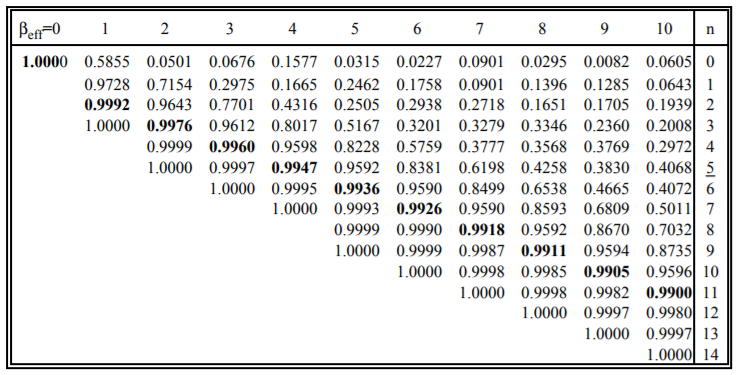
\includegraphics[width=.55\linewidth]{graphics/14.png}
	\caption{En lydbølges refleksioner sker både som en direkte spejling af lydbølgen og som en diffus lydbølge.}
	\label{fig:14}
\end{figure}

\subsubsection{Diffraktion}
Hvordan lydbølger bøjes af små forhindringer og hvordan lydbølger udbredes efter små åbninger. 

\begin{itemize}
	\item En forhindring meget smallere end lydbølgen gør at lydbølgen kan passere uden at blive synderligt forstyrret.
	\item En forhindring større end lydbølgen vil resultere i at der bliver kastet en skygge (casts a shadow) der vil  blive bestrålet fra kilder, der går forbi forhindringen.
\end{itemize}

\begin{figure} [H]
	\centering
	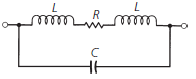
\includegraphics[width=.5\linewidth]{graphics/15.png}
	\caption{Diffraktion er wavelength-dependent.}
	\label{fig:15}
\end{figure}

\begin{itemize}
	\item Diffraktionen afhænger af	den relative størrelse af åbningen. 
	\item En stor åbning med hensyn til bølgelængde tillader lydbølger at gå igennem med en lille forstyrrelse. 
	\begin{itemize}
		\item Disse bølgefronter virker som nye kilder, der udstråler lydenergi i skyggezonen.
	\end{itemize}
	\item Hvis åbningen er lille i forhold til bølgelængden, vil de små bølgefronter, der trænger ind i åbningen virke som punktkilder.
	\begin{itemize}
		\item Disse små bølgefronter vil udstråle et halvkugleformet lydfelt ind i skyggezonen.
	\end{itemize} 
\end{itemize}

\begin{figure} [H]
	\centering
	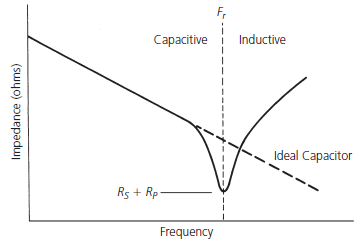
\includegraphics[width=.5\linewidth]{graphics/16.png}
	\caption{Lydbølger der rammer en barriere med en åbning.}
	\label{fig:16}
\end{figure}


\subsection{Statistisk rumakustik}
\begin{itemize}
	\item Antager at lydenergien er konstant overalt i rummet.
	\item \textbf{Sabines formel} for efterklangstiden $T_{60}$ som funktion af rummets volumen V og det lydabsorberende areal S.
\end{itemize}

\begin{equation}
T_{60} = \ln(10^6)\dfrac{4V}{S c} = 55.3\dfrac{V}{S c} = 0.16\dfrac{V}{S}
\end{equation}

\begin{itemize}
	\item For lyddæmpede rum giver Sabines formel en efterklangstid selv om der ikke er refleksioner. En modificeret udgave af Sabines formel blev udledt af Eyring.
	\item \textbf{Eyrings formel} er modificeret ud fra geometriske betragtninger.
\end{itemize}

\begin{equation}
T_{60} = 0.16\dfrac{V}{4 m V-S\ln(1-\alpha)}
\end{equation}

\begin{description}
	\item[$\alpha$] $=\frac{1}{S}\sum_{n}^{}S_n \alpha_n$
	\item[$m$] $\approx0.0011 m^{–1}$ ved \SI{1}{\kilo\hertz}, \SI{20}{\degreeCelsius} og 60 \% relativ luftfugtighed
\end{description}
\textit{m} kan ignoreres for mindre rum og rum med ringe dæmpning bliver formlen lig med Sabines.

\subsection{Absorptionskoeffficienter}
\begin{itemize}
	\item Typisk opsætning af lydabsorberende skumplast og Rockwool er direkte på en hård betonvæg.
	\item Tykkelsen er afgørende for hvor lave frekvenser der kan dæmpes da partikelhastigheden er nul ved væggen så det er kun	ved høje frekvenser at der er bevægelse i luften inde i materialet.
	\item For at opnå større absorption ved lave frekvenser kan benyttes absorbere baseret på en membran.
	\begin{itemize}
		\item De består af en plade eller film af træ, plast eller metal som lydtrykket får til at vibrere.
		\item Derved skal luften bag ved membranen også svinge så luften presses igennem det absorberende materiale.
	\end{itemize}
\end{itemize}


\chapter{Opgaver}
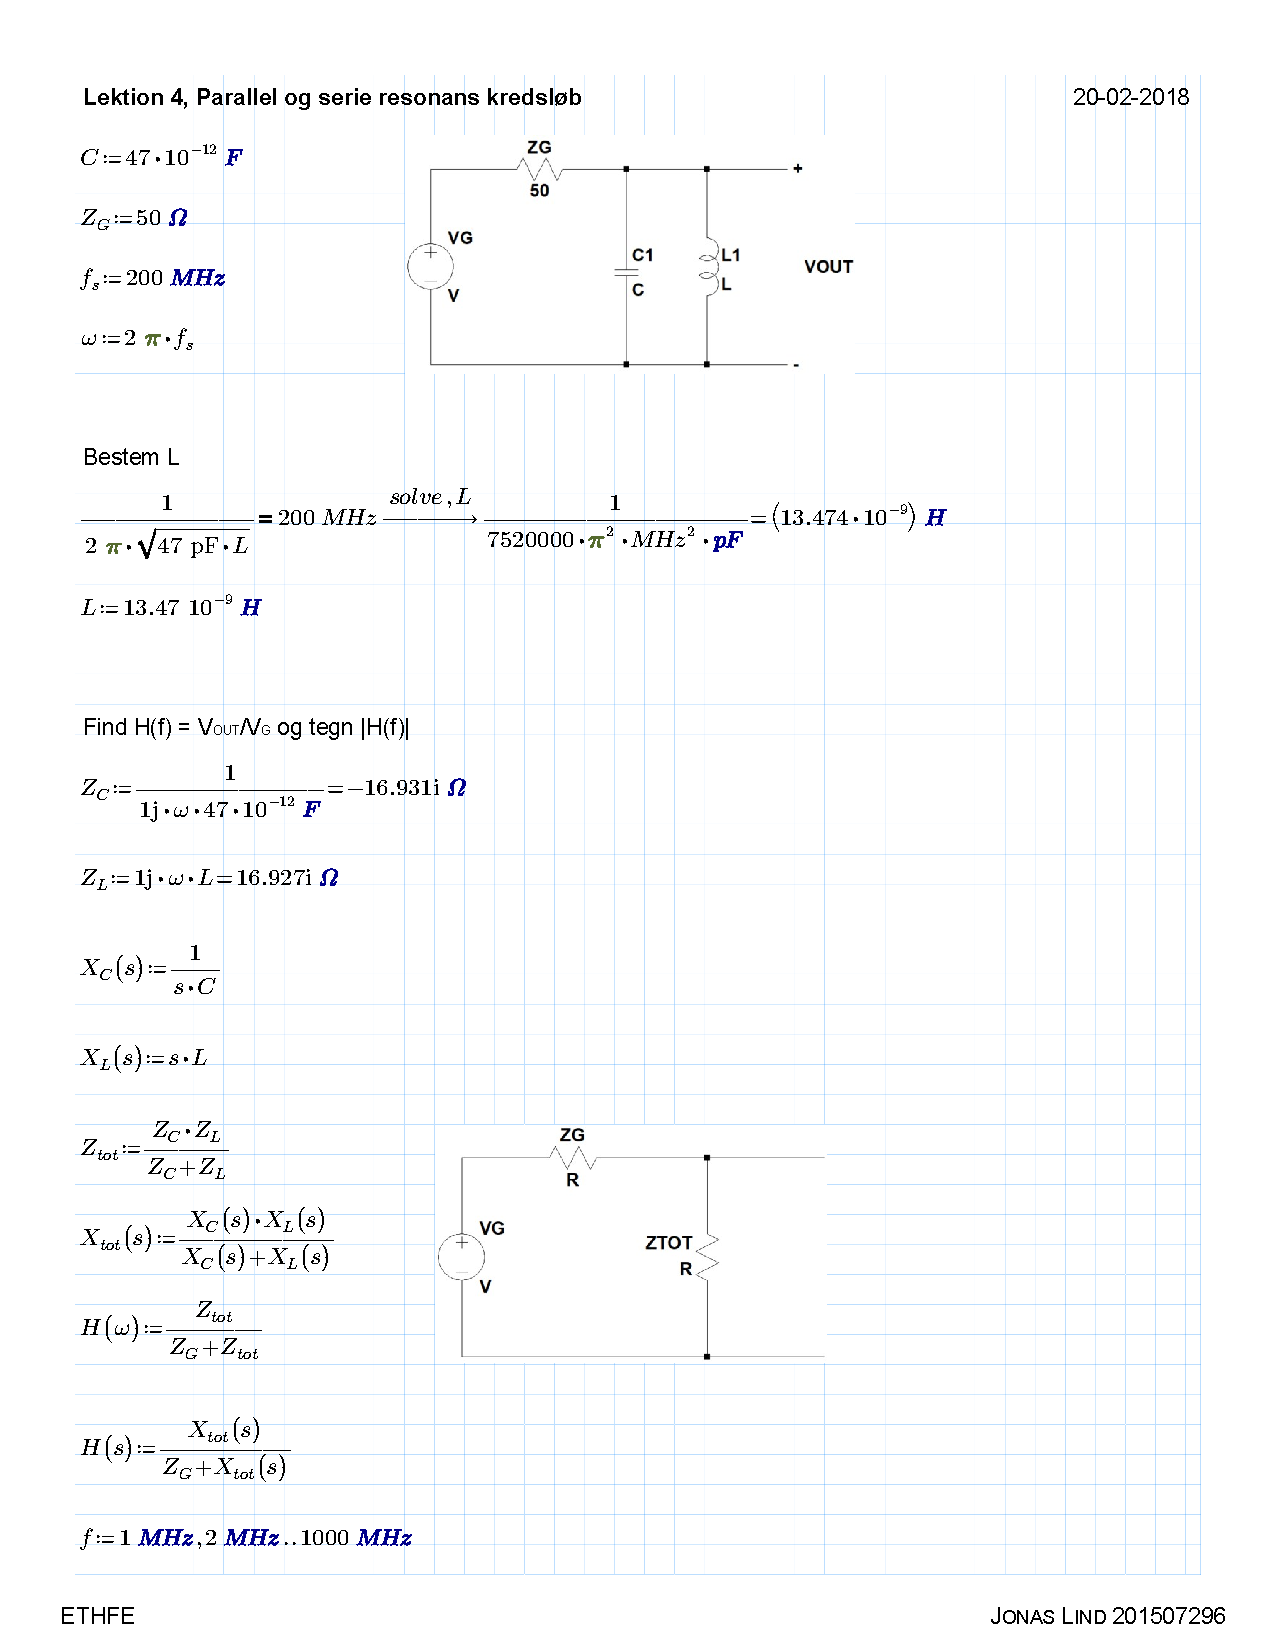
\includepdf[pages=-]{tasks/ETHFE_Lektion4.pdf}
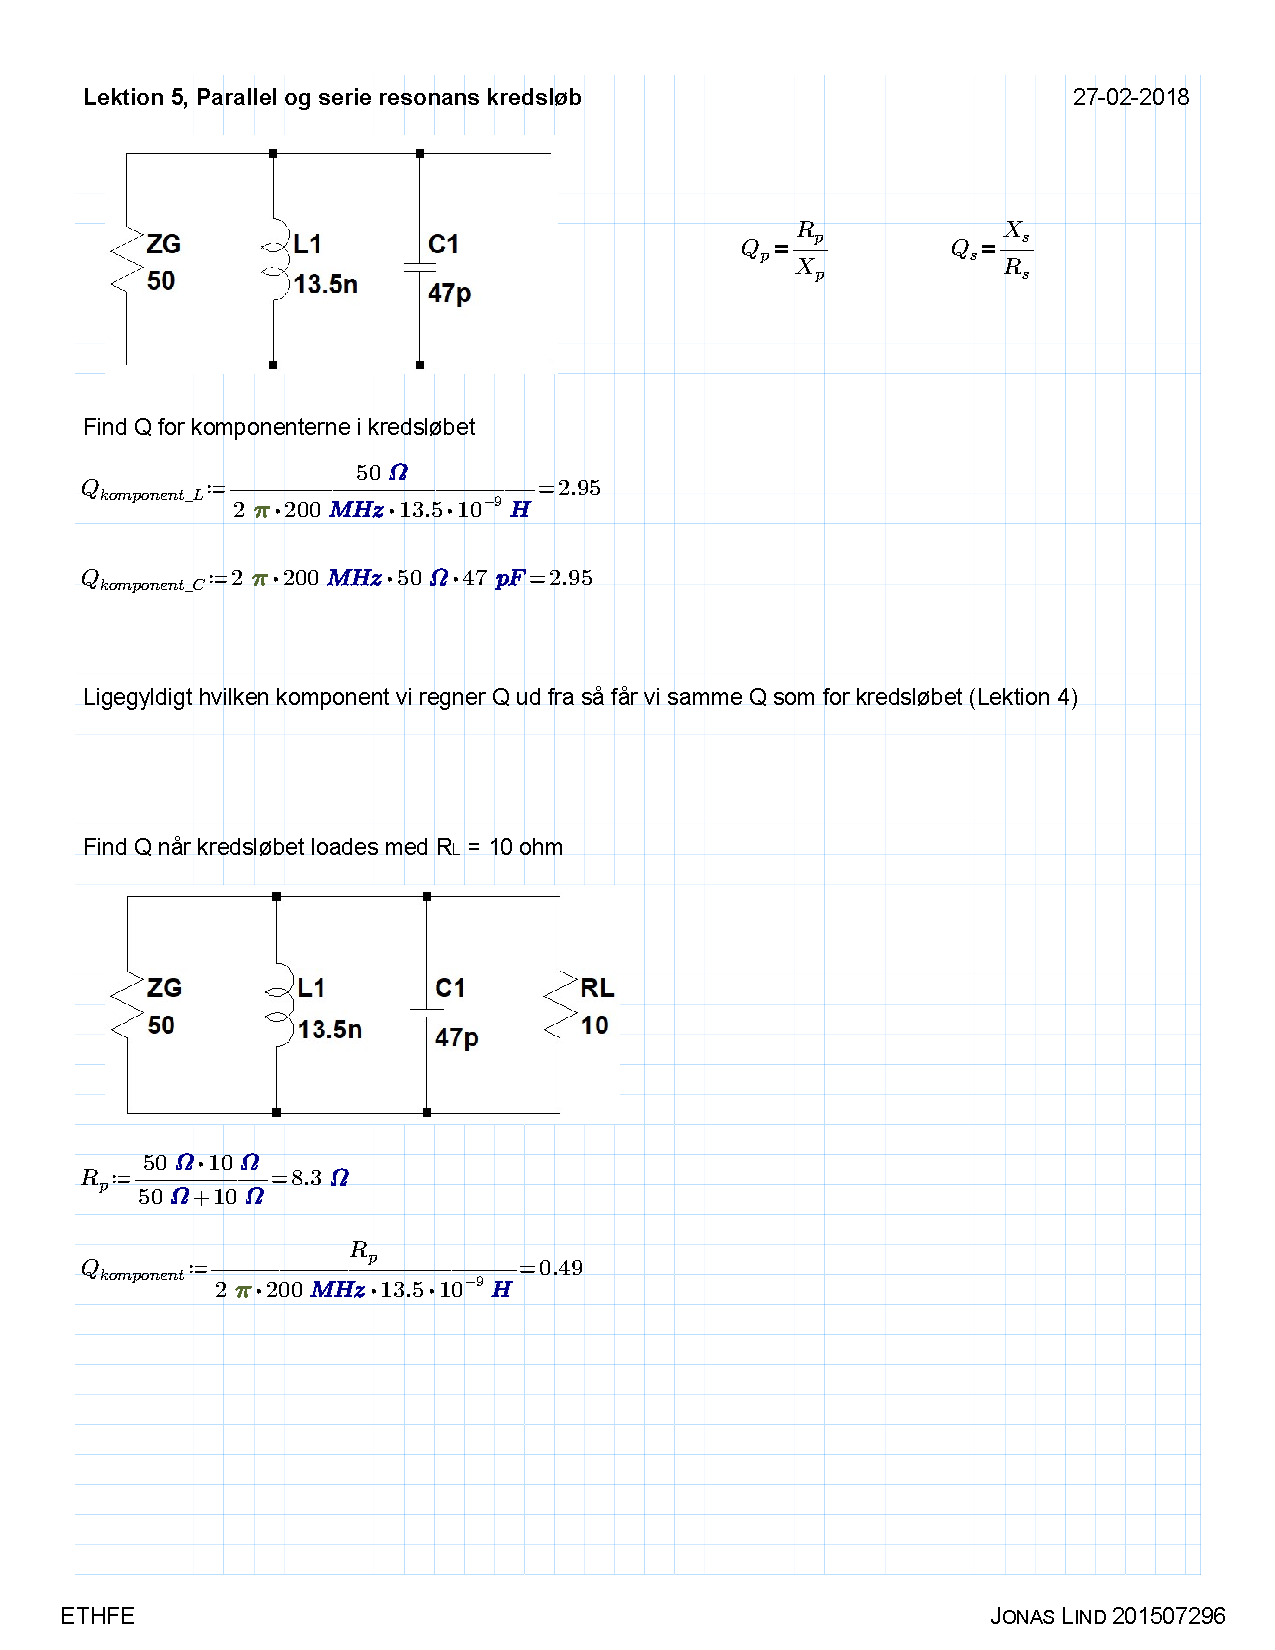
\includepdf[pages=-]{tasks/ETHFE_Lektion5.pdf}

\end{document}